\documentclass[epj, draft]{svjour}

% Packages
\usepackage{latexsym}
\usepackage{graphicx}
\usepackage{hyperref} % provide links in pdf
\usepackage[english]{babel}
\usepackage[utf8]{inputenc}
\usepackage{xcolor}
\usepackage{amsmath}
\usepackage{amstext}
\usepackage{url}
\usepackage[english]{babel}
\usepackage{booktabs}
\usepackage{threeparttable}
\usepackage[title]{appendix}
\usepackage{pdflscape}
\usepackage{afterpage}

\hypersetup{%
   	pdfpagelabels=true,%
	plainpages=false,%
	pdfauthor={J. Henao-Londono et al.},%
	pdftitle={Price response functions and spread impact in correlated
			  financial markets},%
	pdfsubject={Complex Systems},%
	bookmarksnumbered=true,%
	colorlinks=true,%
	citecolor=blue,%
	filecolor=black,%
	linkcolor=blue,% you should probably change this to black before printing
	urlcolor=blue,%
	pdfstartview=FitH%
}

\begin{document}

% Title
\title{Response functions and spread impact in correlated financial markets}
% Authors
\author{Juan C. Henao-Londono
        \thanks{\emph{e-mail: }\href{mailto:juan.henao-londono@uni-due.de}
        {juan.henao-londono@uni-due.de}}
        \and Sebastian M. Krause
        \and Thomas Guhr}
\authorrunning{J. C. Henao-Londono et al.}
% Institute - University
\institute{Fakultät für Physik, Universität Duisburg-Essen, Lotharstraße 1,
           47048 Duisburg, Germany}
% Date
\date{Received: date / Revised version: date}

\abstract{
Insert your abstract here.
\PACS{
      {89.65.Gh}{Econophysics} \and
      {89.75.-k}{Complex systems} \and
      {05.10.Gg}{Statistical physics}
     } % end of PACS codes
} %end of abstract

\maketitle

\section{Possible paper names (I will erase this when we choose a name)}
The following are possible names for the paper:

\begin{itemize}
  \item Details that influence the response functions results.
  \item Influence of the details in the response function measurement.
  \item Response function measurement in correlated financial markets.
  \item Response function calculation in correlated financial markets.
  \item Influence of the methodology in response functions results.
\end{itemize}

Or we can use another.

\section{Introduction}\label{sec:introduction}

Financial markets use order books to list the number of shares bid or asked at
each price. An order book is an electronic list of buy and sell orders for a
specific security or financial instrument organized by price level, agents can
place different types of instructions (orders).

In general, the dynamics of the prices follow a random walk. There are two
extreme models that can describe this behavior: the Efficient Market Hypothesis
(EMH) and the Zero Intelligence Trading (ZIT). The EMH states that all
available information is included in the price and price changes can only be
the result of unanticipated news, which by definition are totally unpredictable
\cite{subtle_nature,Bouchaud_2004,EMH_lillo,stat_theory}. On the other hand,
the ZIT assumes that agents instead of being fully rational, have ``zero
intelligence” and randomly buy or sell. It is supposed that their actions are
interpreted by other agents as potentially containing some information
\cite{subtle_nature,Bouchaud_2004,stat_theory,Wang_2016_cross}.
In both cases the outcome is the same, the prices follow a random walk. Reality
is somewhere in-between \cite{Bouchaud_2004,stat_theory}, and non-Markovian
effects due to stategies or liquidity costs are not contained either.

There are diverse studies focused on the price response
\cite{dissecting_cross,r_walks_liquidity,subtle_nature,Bouchaud_2004,large_prices_changes,pow_law_dist,theory_market_impact,spread_changes_affect,master_curve,EMH_lillo,quant_stock_price_response,ori_pow_law,prop_order_book,Wang_2018_b,Wang_2018_a,Wang_2016_avg,Wang_2016_cross},
In our opinion, a critical investigation of definitions and methods and how
they affect the results is called for.

Regarding price self-response functions
\cite{r_walks_liquidity,subtle_nature,Bouchaud_2004}, Bouchaud et al. found an
increase to a maximum followed by a decrease as the time lag grows.
In Ref. \cite{theory_market_impact}, Gerig found that larger sized transactions
have a larger absolute impact than smaller sized transactions but a much
smaller relative impact. In Ref. \cite{prop_order_book}, it is found that the
impact of small trades on the price is, in relative terms, much larger than
that of large trades and the impact of trading on the price is quasi-permanent.

For price cross-responses functions, Refs.
\cite{dissecting_cross,Wang_2016_cross} found that the diagonal terms are on
average larger than the off-diagonal ones by a factor $\sim 5$. The response at
positive times is roughly constant, what is consistent with the hypothesis of a
statistically efficient price. Thus, the current sign does not predict future
returns. In Ref. \cite{Wang_2016_cross} the trends in the cross-responses were
found not to depend on whether or not the stock pairs are in the same economic
sector or extend over two sectors.


Here, we want to discuss, based on a series of detailed empirical results
obtained on trade by trade data, that the variation in the details of the
parameters used in the price response definition modify the characteristics of
the results. Aspects like time scale, time shift, time lag and spread used in
the price response calculation have an influence on the outcomes.

We delve into the key details needed to compute the price response functions,
and explore their corresponding roles. We perform a empirical study in
different time scales and find that using different implementations of the
price response, the results are qualitatively the same, but the response can
vary up to a factor of two. We show that the order between the trade signs and
the returns have a key importance in the price response signal and suggest an
interval where the time shift have to be set. We split the time lag to
understand the contribution of the immediate returns and the late returns. The
price response is highly influenced by the instantaneous returns and as the
time lag grows, the influence starts to decrease. We shed light on the spread
impact in the response functions for single stocks. We check that when the
spread is large, the price response tend to be large.

A direct comparison between the trade time scale and the physical time scale is
not possible. To compare them directly we need to assume whether the midpoint
price or the trade signs are on the same scale. We assume the midpoint prices
in the trade time scale to be the same as the midpoint prices in physical time
scale. Therefore, we have the time lag for both computations in seconds. This
approximation allow us to directly compare both scales to have an idea of the
difference and similarities they have. In the other sections, as we are not
directly comparing the time scales, the corresponding quantities of each time
scale are not mixed. Thus physical time scale is measured in seconds and trade
time scale is measured in trades.

The paper is organized as follows: in Sect. \ref{sec:data} we present our data
set of stocks. We then analyze the definition of the price response functions
and describe the physical and trade time in Sect.
\ref{sec:response_functions_def}. We implement different price responses for
several stocks and pairs of stocks in Sect. \ref{sec:response_functions_imp}.
In Sect. \ref{sec:time_shift} we show how the relative position between trade
signs and returns has a huge influence in the results of the computation of the
response functions. In Sect. \ref{sec:short_long} we explain in detail how the
time lag $\tau$ behaves in the response functions. Finally, in Sect.
\ref{sec:spread_impact} we analyze the spread impact in the price response
functions. Our conclusions follow in Sect. \ref{sec:conclusion}.
\section{Data set and time definition}\label{sec:data_time}

In Sect. \ref{subsec:data_set} we introduce the data set used in the paper. In
Sect. \ref{subsec:time_definition} we describe the physical time scale and the
trade time scale.

%%%%%%%%%%%%%%%%%%%%%%%%%%%%%%%%%%%%%%%%%%%%%%%%%%%%%%%%%%%%%%%%%%%%%%%%%%%%%%%
\subsection{Data set}\label{subsec:data_set}

In this study, we have analyzed trades and quotes (TAQ) data from the NASDAQ
Stock Market. We selected NASDAQ because it is an electronic exchange where
stocks are traded through an automated network of computers instead of a
trading floor, which makes trading more efficient, fast and accurate.
NASDAQ is the second largest stock exchange based on market capitalization in
the world.

In the TAQ data set, there are two data files for each stock. One gives the
list of all successive quotes. Thus, we have the best bid price, best ask
price, available volume and the time stamp accurate to the second. The other
data file is the list of all successive trades, with the traded price, traded
volume and time stamp accurate to the second. Despite the one second accuracy
of the time stamps, in both files more than one quote or trade may be recorded
in the same second.

Due to the the time stamp accuracy, it is not possible to match each trade with
the directly preceding quote. Hence, we cannot determine the trade sign by
comparing the traded price and the preceding midpoint price
\cite{Wang_2016_cross}. In this case we need to do a preprocessing of the data
to relate the midpoint prices with the trade signs in trade time scale and in
physical time scale. Observe that we will not be discussing the returns, but
the midpoint price. This because both are intrinsically related, as explained
before, and it is more intuitive to understand the changes in midpoint prices
than in returns.

To analyze the response functions across different liquid stocks, we select the
six companies with the largest average market capitalization (AMC) (Alphabet
Inc., Mastercard Inc., CME Group Inc., Goldman Sachs Group Inc., Transocean
Ltd. and Apache Corp.) in three economic sectors (information technology,
financials and energy) of the S\&P index in 2008.

In order to avoid overnight effects and any artifact due to the opening and
closing of the market, we systematically discarded the first ten and the last
ten minutes of trading in a given day
\cite{Bouchaud_2004,large_prices_changes,spread_changes_affect,Wang_2016_cross}.
Therefore, we only consider trades of the same day from 9:40:00 to 15:50:00
New York local time. We will refer to this interval of time as the ``market
time".


\begin{table*}[htbp]
\begin{threeparttable}
\caption{Analyzed companies.}
\begin{tabular*}{\textwidth}{c @{\extracolsep{\fill}} ccccc}
\toprule
\bf{Company} & \bf{Symbol} & \bf{Sector} & \bf{Quotes}\tnote{1} &
\bf{Trades}\tnote{2} & \bf{Spread}\tnote{3}\tabularnewline
\midrule
Alphabet Inc. & GOOG & Information Technology (IT) & $164489$ & $19029$ &
$\$0.04$\tabularnewline
Mastercard Inc. & MA & Information Technology (IT) & $98909$ & $6977$ &
$\$0.38$\tabularnewline
CME Group Inc. & CME & Financials (F) & $98188$ & $3032$ &
$\$1.08$\tabularnewline
Goldman Sachs Group Inc. & GS & Financials (F) & $160470$ & $26227$ &
$\$0.11$\tabularnewline
Transocean Ltd. & RIG & Energy (E) & $107092$ & $11641$ &
$\$0.12$\tabularnewline
Apache Corp. & APA & Energy (E) & $103074$ & $8889$ & $\$0.13$\tabularnewline
\bottomrule
\end{tabular*}
\label{tab:companies}
\begin{tablenotes}\footnotesize
\item[1] Average number of quotes from 9:40:00 to 15:50:00 New York time.
\item[2] Average number of trades from 9:40:00 to 15:50:00 New York time.
\item[3] Average spread from 9:40:00 to 15:50:00 New York time.
\end{tablenotes}
\end{threeparttable}
\end{table*}

Table \ref{tab:companies} shows the companies analyzed with their corresponding
symbol and sector. The highest average number of quotes per day and the most
liquid stock on average from our selection for the year 2008 is Alphabet Inc.
The most traded stock on average from the group was Goldam Sachs Group Inc.
On the other side, the stock with the less quotes, less traded and less
liquidity on average for the analyzed year was CME Group Inc.

%%%%%%%%%%%%%%%%%%%%%%%%%%%%%%%%%%%%%%%%%%%%%%%%%%%%%%%%%%%%%%%%%%%%%%%%%%%%%%%
\subsection{Time definition}\label{subsec:time_definition}

A key concept in the analysis of the response functions is the time. Due to the
nature of the data, they are several options to define the time.

In general, the time series are indexed in calendar time (hours, minutes,
seconds, milliseconds). Moreover, tick-by-tick data available on financial
markets all over the world is time stamped up to the millisecond, but the order
of magnitude of the guaranteed precision is much larger, usually one second or
a few hundreds of milliseconds \cite{empirical_facts}. In several papers are
used different time definitions (calendar time, physical time, event time,
trade time, tick time) \cite{empirical_facts,sampling_returns,market_making}.
The TAQ data used in the analysis has the characteristic that the trades and
quotes can not be directly related due to the time stamp resolution of only one
second \cite{Wang_2016_cross}. Hence, it is impossible to match each trade with
the directly preceding quote. However, using a classification for the trade
signs, we can compute trade signs in two scales: trade time scale and physical
time scale.

The trade time scale is increased by one unit each time a transaction happens.
The advantage of this count is that limit orders far away in the order book do
not increase the time by one unit. The main outcome of trade time scale is its
``smoothing" of data and the aggregational normality \cite{empirical_facts}.

The physical time scale is increased by one unit each time a second passes.
This means that computing the responses in this scale involves sampling
\cite{sampling_returns,Wang_2016_cross}, which has to be done carefully when
dealing for example with several stocks with different liquidity. This sampling
is made in the trade signs and in the midpoint prices.

Facing the impossibility to relate midpoint prices and trade signs with the TAQ
data in trade time scale, we will use the midpoint price of the previous second
with all the trade signs of the current second. This will be our definition of
trade time scale analysis for the response function analysis.

For physical time scale, as we can sampling, we relate the unique value of
midpoint price of a previous second with the unique trade sign value of the
current second.

Thus, trade sign values will be used in trade time scale and physical time
scale and returns will be only used in physical time scale.

%%%%%%%%%%%%%%%%%%%%%%%%%%%%%%%%%%%%%%%%%%%%%%%%%%%%%%%%%%%%%%%%%%%%%%%%%%%%%%%
\subsubsection{Trade time scale}\label{subsubsec:trade_time}

We use the trade sign classification in trade time scale proposed by S. Wang et
al. in \cite{Wang_2016_cross} and used in
\cite{Wang_2017,Wang_2018_copulas,Wang_2016_avg} that reads

\begin{equation}\label{eq:trade_signs_trade}
    \varepsilon^{t}\left(t,n\right)=\left\{
    \begin{array}{cc}
    \text{sgn}\left(S\left(t,n\right)-S\left(t,n-1\right)\right),
    & \text{if }\\ S\left(t,n\right) \ne S\left(t,n-1\right)\\
    \varepsilon\left(t,n-1\right),
    & \text{otherwise}
    \end{array}\right.
\end{equation}

$\varepsilon^{t}\left( t,n \right) = +1$ implies a trade triggered by a market
order to buy, and a value $\varepsilon^{t}\left( t,n \right) = -1$ indicates a
trade triggered by a market order to sell.

In the second case of the classification, if two consecutive trades with the
same trading direction did not exhaust all the available volume at the best
quote, the trades would have the same price, and in consequence they will have
the same trade sign.

With this classification we obtain trade signs for every single trade in the
data set. According to \cite{Wang_2016_cross}, the average accuracy of the
classification is $85\%$ for the trade time scale.

TAQ time step is one second, and as it is impossible to find the
correspondences between trades and midpoint prices values inside a second step,
We used the last midpoint price of every second as the representative value of
each second. This introduce an apparent shift between trade signs and returns.
In fact, we set the last midpoint price from the previous second as the first
midpoint price of the current second, as explained in \cite{Wang_2016_cross}.

As we know the second in which the trades were made, we can relate the trade
signs and the midpoint prices as shown in Fig.
\ref{fig:relation_trades_midpoint_trade_scale}. For the trade time scale, they
are in general, several midpoint prices in a second. For each second we
select the last midpoint price value, and we relate it to the next second
trades. In Fig. \ref{fig:relation_trades_midpoint_trade_scale}, the last
midpoint price (circle) between the second $-1$ and $0$ is related with all the
trades (squares and triangles) in the second $0$ to $1$, and so on. It is worth
to note, in the seconds that there are no changes in the quotes, it is used the
value of the previous second (vertical line over the physical time interval).
Thus, all the seconds in the open market time have a midpoint price value, and
in consequence returns values. We assume that as there was not a change in the
quotes, the midpoint price remain the same as the last one.

\begin{figure}[htbp]
    \centering
    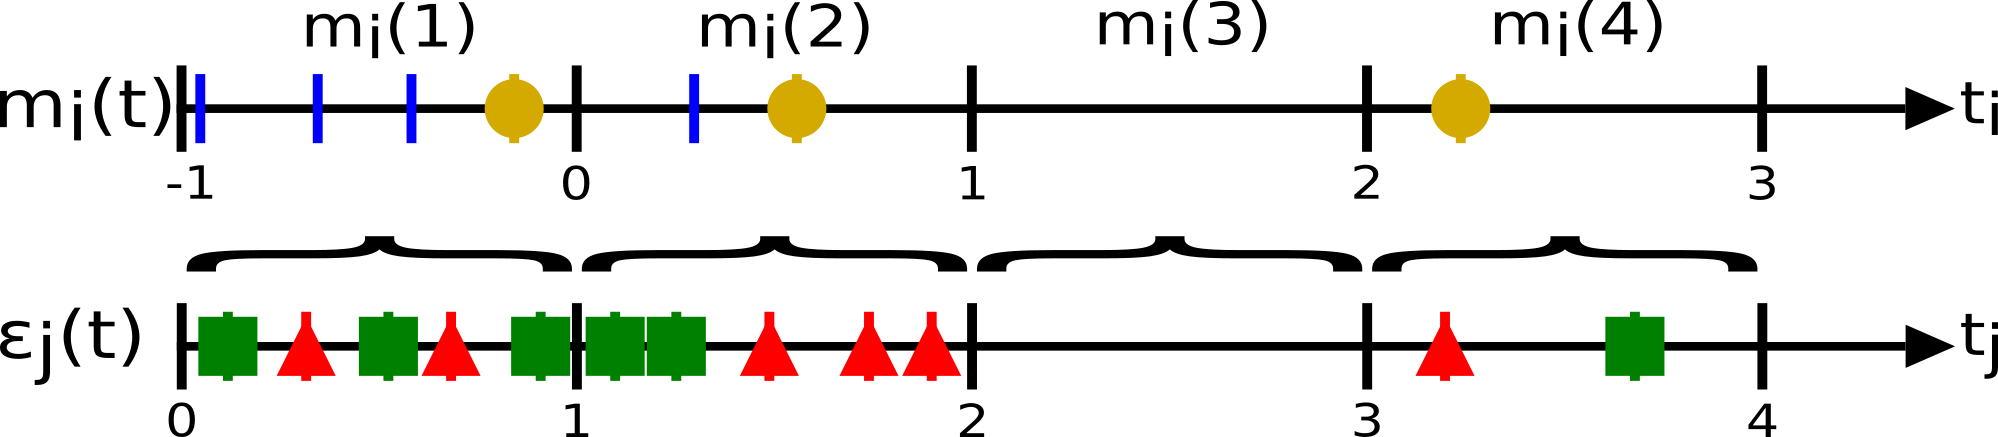
\includegraphics[width=\columnwidth]
    {figures/02_relation_trades_quotes_trade_scale.png}
    \caption{Sketch of data processing for trade time scale. In the midpoint
             price time line, the vertical lines represent the change in price
             of the quotes and the circles represent the last price change in a
             quote in a second. In the trade signs time line, the squares
             represent the buy market orders and the triangles represent the
             sell market orders. The midpoint price time line and the trade
             sign time line are shifted in one second.}
    \label{fig:relation_trades_midpoint_trade_scale}
\end{figure}

We computed all the analysis for the trade time scale using Equations
\ref{eq:midpoint_price_return} and \ref{eq:trade_signs_trade}.

The methodology described is an approximation to compute the response in the
trade time scale. A drawback in the computation could come from the fact that
the return of a given second is composed by the contribution of small returns
corresponding to each change in the midpoint price during a second. As we are
assuming only one value for the returns in each second, we are supposing  all
the returns in one second interval to be positive or negative, which could not
be the case. This could increase or decrease the response signal at the end of
the computation.

\begin{figure}[htbp]
    \centering
    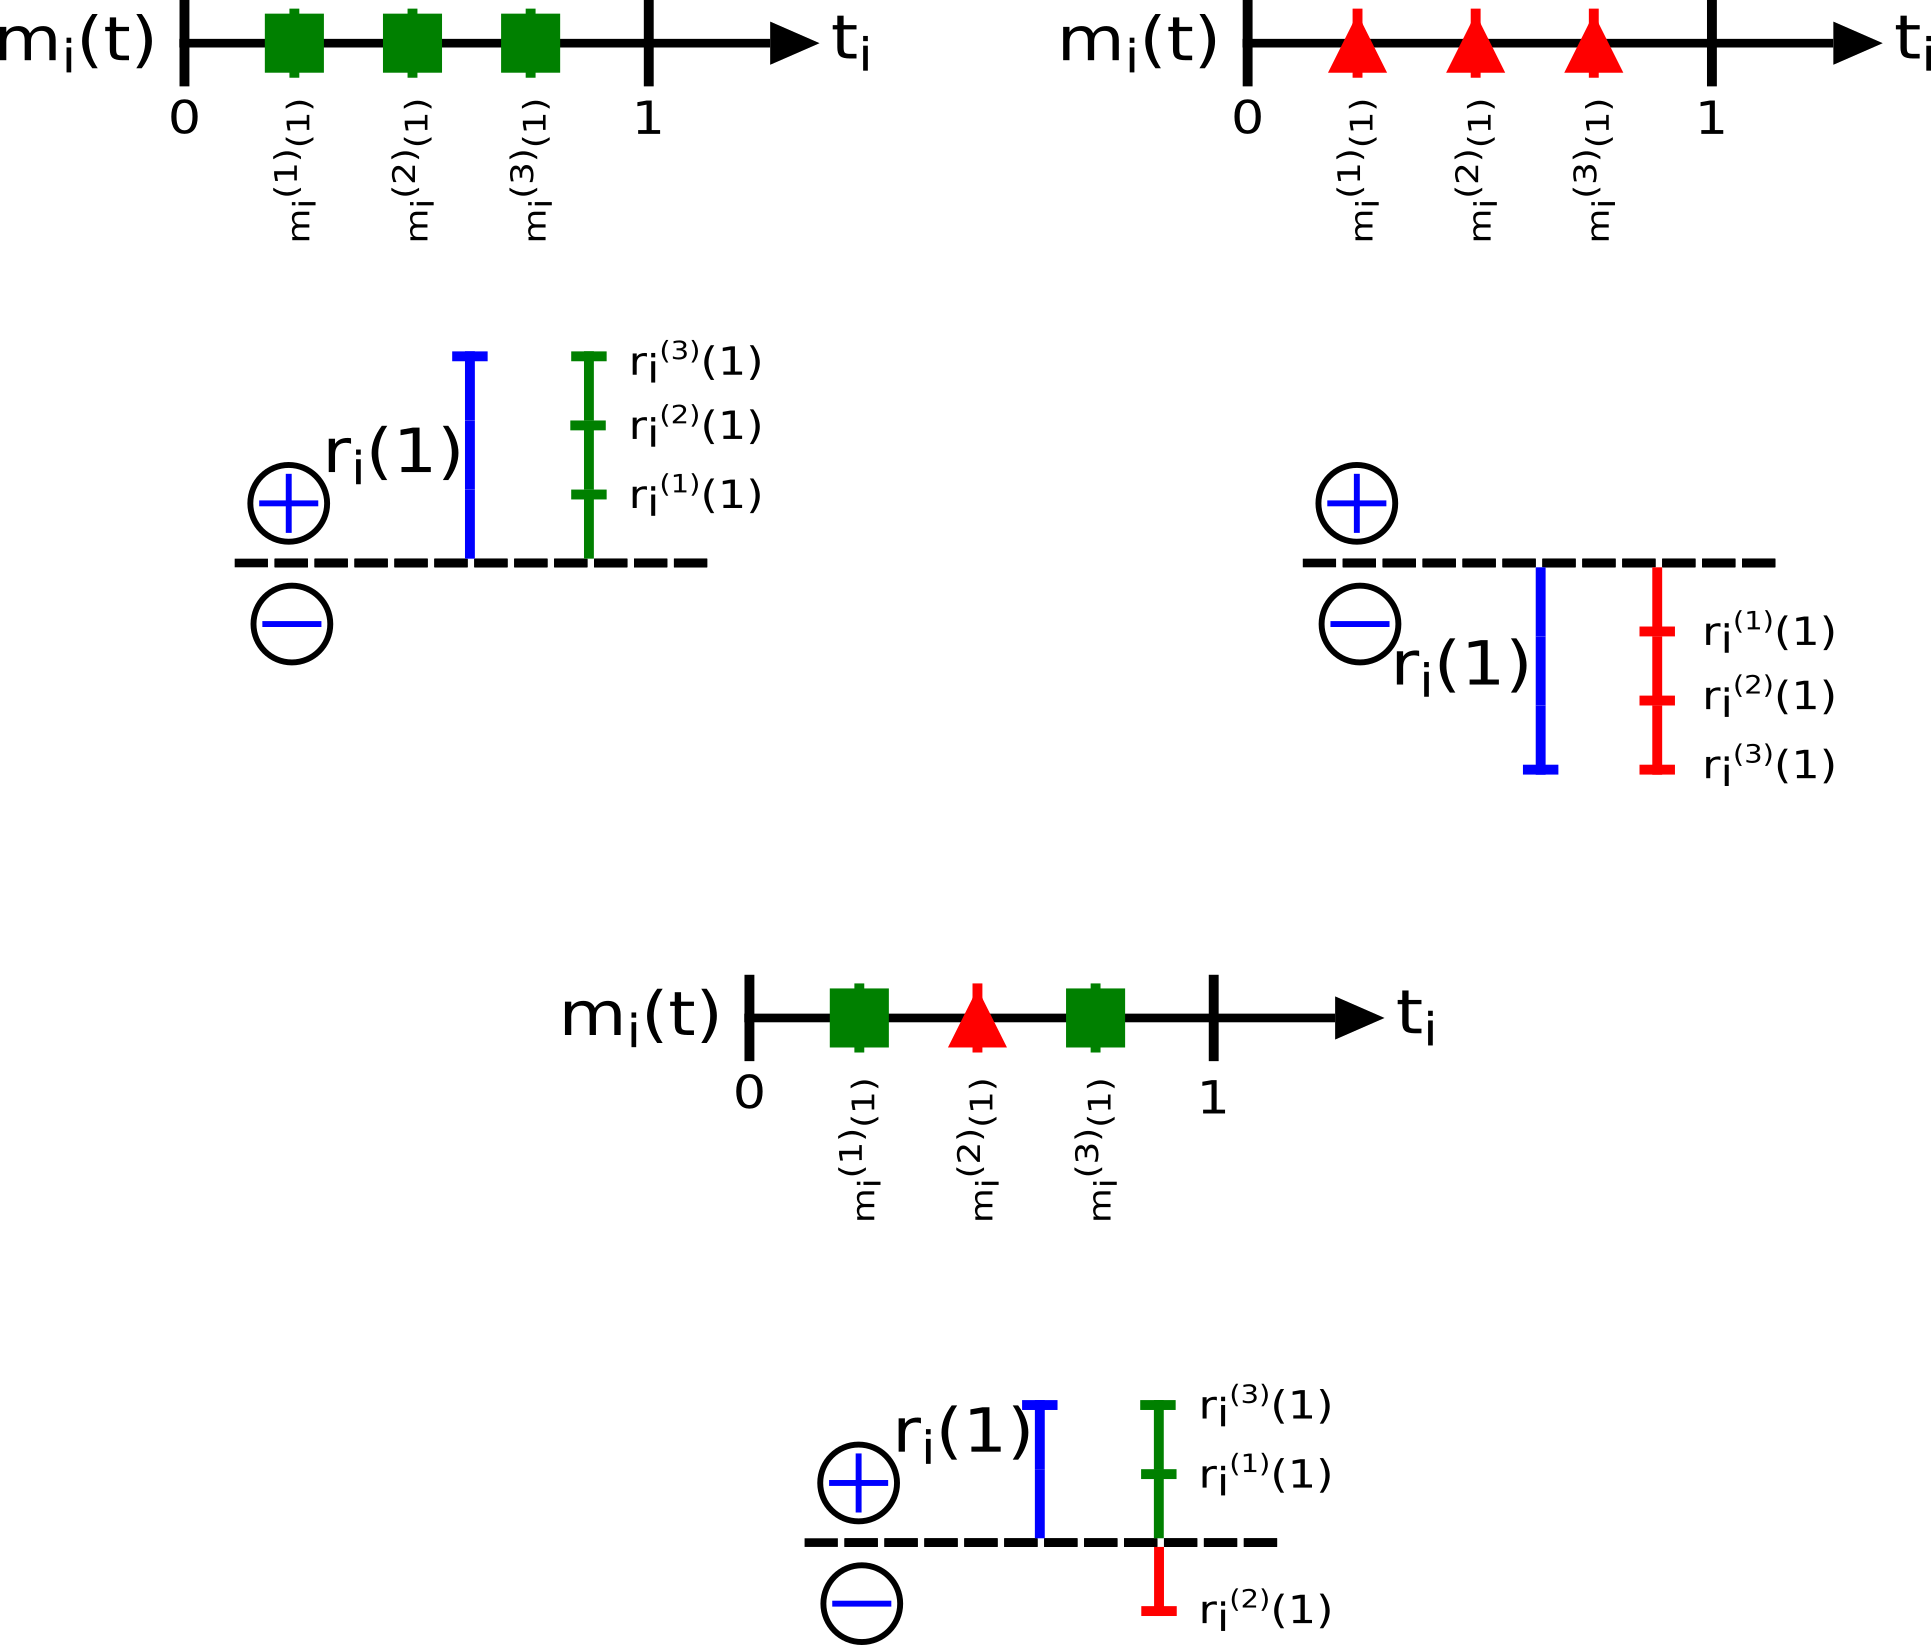
\includegraphics[width=\columnwidth]{figures/02_return_contributions.png}
    \caption{Sketch of the return contributions from every midpoint price
             change in a second. The squares represent the rise of the price of
             the midpoint price and the triangles represent the decrease of the
             price of the midpoint price. We illustrate three cases: (top left)
             the changes of the midpoint prices and return are due to the rise
             of the prices, (top right) the changes of the midpoint prices and
             return are due to the decrease of the prices, and (bottom) the
             changes of the midpoint prices and return are due to a combination
             of rise and decrease of the prices.}
    \label{fig:return_contributions}
\end{figure}

Figure \ref{fig:return_contributions} illustrate with one example this point.
Suppose one second interval, in which they are three different midpoint prices,
and as result, three different returns for this three midpoint price
values. Furthermore, consider that the volume of limit orders that have the
corresponding midpoint price are the same in the bid and in the ask (so the
impact have the same magnitude). In the case of the top left (top right)
sketch, all the changes are due to the rise (decrease) of the midpoint price,
that means, consumption of the best ask (bid), so all the contributions of the
individual returns in the second are positive (negative), and in repercussion,
the net return is positive (negative). In the case of the bottom, the changes
are due to a combination of increase and decrease of the midpoint price, so in
the end the individual returns sum up to a net return, which can be positive or
negative, depending of the type of midpoint price values in the interval. Thus,
in this case, we are assuming at the end that all the returns were positive or
negative, what probably was not the case, and in consequence will increase or
decrease the real value of the net return.

In all the cases we choose the last change in the midpoint price in a second
interval as described before
(Fig. \ref{fig:relation_trades_midpoint_trade_scale}). We use this method
knowing that the variation in one second of the midpoint price is not large
(in average, the last midpoint price of a second differ with the average
midpoint of that second in $0.007\%$), so it can give us valuable information
about the response functions.

%%%%%%%%%%%%%%%%%%%%%%%%%%%%%%%%%%%%%%%%%%%%%%%%%%%%%%%%%%%%%%%%%%%%%%%%%%%%%%%
\subsubsection{Physical time scale}\label{subsubsec:physical_time}

We use the trade sign definition in physical time scale proposed by
S. Wang et al. in \cite{Wang_2016_cross} and used in
\cite{Wang_2017,Wang_2016_avg}, that depends on the classification in
Eq. \ref{eq:trade_signs_trade} and reads

\begin{equation}\label{eq:trade_signs_physical}
    \varepsilon^{p}\left(t\right)=\left\{
    \begin{array}{cc}
    \text{sgn}\left(\sum_{n=1}^{N\left(t\right)}\varepsilon^{t}
    \left(t,n\right)\right),
    & \text{If }N \left(t\right)>0\\
    0, & \text{If }N\left(t\right)=0
    \end{array}\right.
\end{equation}

Where $N \left(t \right)$ is the number of trades in a second interval.
$\varepsilon^{p}\left( t \right) = +1$ implies that the majority of
trades in second $t$ were triggered by a market order to buy, and a value
$\varepsilon^{p}\left( t \right) = -1$ indicates a majority of sell
market orders. In this definition, they are two ways to obtain
$\varepsilon^{p}\left( t \right) = 0$. One way is that in a particular
second there is not trades, and then no trade sign. The other  way is that the
addition of the trade signs ($+1$ and $-1$) in a second be equal to zero. In
this case, there is a balance of buy and sell market orders.

Market orders show opposite trade directions to limit order executed
simultaneously. An executed sell limit order corresponds to a buyer-initiated
market order. An executed buy limit order corresponds to a seller-initiated
market order.

As in the trade time scale, in the physical time scale we use the same strategy
to obtain the midpoint price for every second, so all the seconds in the open
market time have a midpoint price value. It is worth to note again, that even
if the second does not have a change in quotes, it will has still a midpoint
price value and a return value.

\begin{figure}[htbp]
    \centering
    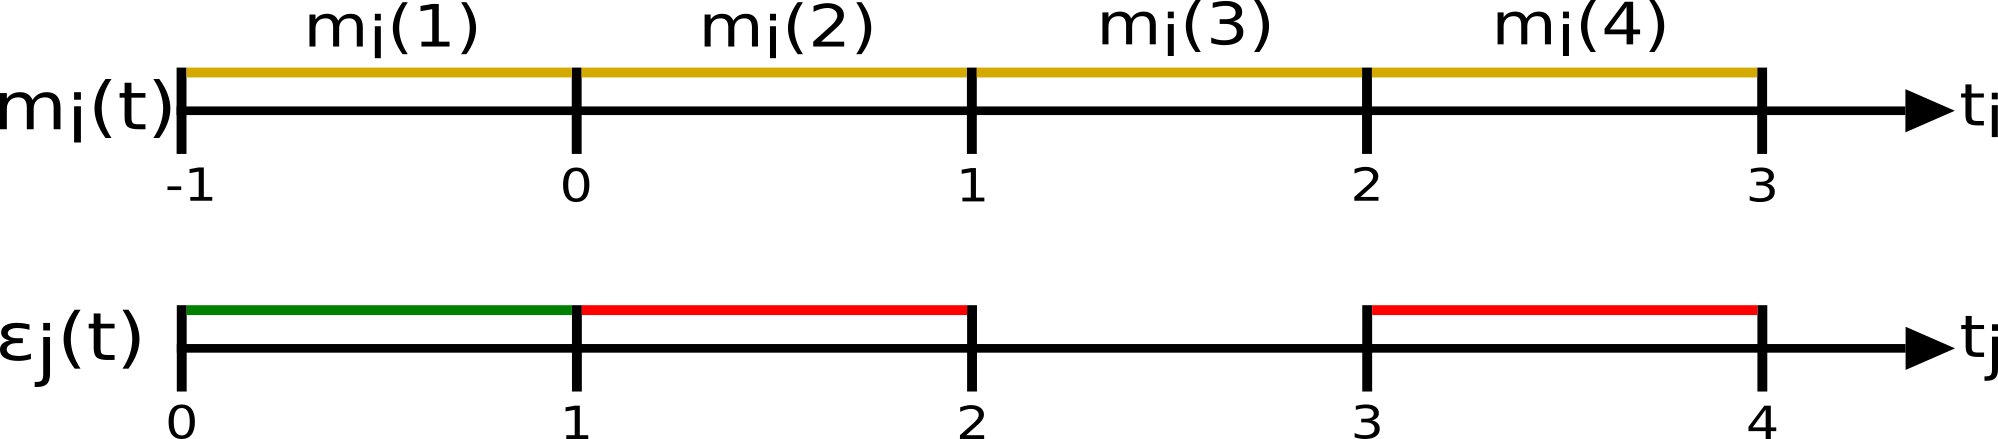
\includegraphics[width=\columnwidth]
    {figures/02_relation_trades_quotes_time_scale.png}
    \caption{Sketch of data processing for physical time scale. In the midpoint
             price time line, the horizontal lines between seconds represent
             the midpoint prices. In the trade signs time line, the horizontal
             lines between seconds represent the trade sign values. The
             midpoint price time line and the trade sign time line are shifted
             in one second.}
    \label{fig:relation_trades_midpoint_time_scale}
\end{figure}

In this case we do not compare every single trade sign in a second, but the net
trade sign obtained for every second with the definition. This can be seen in
Fig. \ref{fig:relation_trades_midpoint_time_scale}, we related the midpoint
price of the previous second with the trade sign of the current second.

According to \cite{Wang_2016_cross}, this definition has an average
accuracy up to $82\%$ in the physical time scale.
\section{Response functions}\label{sec:response_functions}

The main objective of this work is to analyze the response functions. In
general we define the self- and cross-response in a correlated financial market
as

\begin{equation}\label{eq:response_general}
    R^{scale}_{ij}\left(\tau\right)=\left\langle r^{p}_{i}\left(t-1,
    \tau\right) \cdot\varepsilon^{scale}_{j} \left(t\right)\right\rangle
    _{scale}
\end{equation}

where the index $i$ and $j$ correspond to stocks in the market,
$r^{p}_{i}$ is the return of the stock $i$ in a time lag $\tau$ and
$\varepsilon^{scale}_{j}$ is the trade sign of the stock $j$ in the
corresponding scale. The subscript and superscript $scale$ refer to the time
scale used, wheter physical time scale or trade time scale. Finally, we average
the product over the physical time or trade time depending on the time scale.

We use the returns and the trade signs to define three response functions:
trade time scale response, physical time scale response and activity response.

To compare the three response functions, we define the following quantities

\begin{align}
    E_{j,d}\left(t\right)&=\sum_{n=1}^{N\left(t\right)}
    \varepsilon_{j,d}^{t}\left(t,n\right)\\
    E_{j,d}\left(t\right)&=\text{sgn}\left(E_{j,d}\left(t\right)\right)
    \cdot\left|E_{j,d}\left(t\right)\right|\\
    \varepsilon_{j,d}^{p}\left(t\right)&=
    \text{sgn}\left(E_{j,d}\left(t\right)\right)
\end{align}

Where the subscript $d$ refers to the days used in the response computation.

In Sect. \ref{subsec:response_function_trade} we analyze the responses
functions in trade time scale, in Sect. \ref{subsec:response_function_physical}
we analyze the responses functions in trade time scale and in Sect.
\ref{subsec:activity_response_function} we define a response function to
analyze the influence of the frequency of trades in a second.

%%%%%%%%%%%%%%%%%%%%%%%%%%%%%%%%%%%%%%%%%%%%%%%%%%%%%%%%%%%%%%%%%%%%%%%%%%%%%%%
\subsection{Response functions in trade time scale}
\label{subsec:response_function_trade}

We define the self- and cross-response functions in trade time scale, using the
trade signs in trade time scale and the returns in physical time scale. The
response is

\begin{equation}\label{eq:response_functions_trade_scale_general}
    R^{t}_{ij}\left(\tau\right)=\left\langle r^{p}_{i}\left(t-1,\tau
    \right)\cdot\varepsilon_{j}^{t} \left(t, n\right)\right\rangle _{t}
\end{equation}

However, to be explicit with the way the averaging is made, the function reads

\begin{align}\label{eq:response_trades_explicit}
    R_{ij}^{t}\left(\tau\right)&=\frac{1}{\sum_{d=d_{0}}^{d_{f}}
    \sum_{t=t_{0}}^{t_{f}}N_{j,d} \left(t \right)} \nonumber \\
    &\cdot\sum_{d=d_{0}}^{d_{f}}\sum_{t=t_{0}}^{t_{f}}\sum_{n=1}
    ^{N\left(t\right)} r^{p}_{i,d}\left(t-1, \tau\right)\cdot
    \varepsilon_{j,d}^{t}\left(t,n\right)\\
    &=\sum_{d=d_{0}}^{d_{f}}\sum_{t=t_{0}}^{t_{f}} r^{p}_{i,d}
    \left(t-1,\tau\right) \cdot\frac{\sum_{n=1}^{N\left(t\right)}
    \varepsilon_{j,d}^{t}\left(t,n \right)} {\sum_{d=d_{0}}^{d_{f}}
    \sum_{t=t_{0}}^{t_{f}}N_{j,d}\left(t\right)} \nonumber \\
    &=\sum_{d=d_{0}}^{d_{f}}\sum_{t=t_{0}}^{t_{f}}r^{p}_{i,d}
    \left(t-1,\tau\right) \cdot \text{sgn}\left(E_{j,d}\left(t\right)\right)
    \cdot w_{j,d}^{t}\left(t\right)
\end{align}

Where

\begin{equation}\label{eq:trade_weight}
    w_{j,d}^{t}\left(t\right) = \frac{\left|E_{j,d}\left(t\right)\right|}
    {\sum_{d=d_{0}}^{d_{f}}\sum_{t=t_{0}}^{t_{f}}N_{j,d} \left(t\right)}
\end{equation}

is a weight function that depends on the normalization of the response.

\begin{figure*}[htbp]
    \centering
    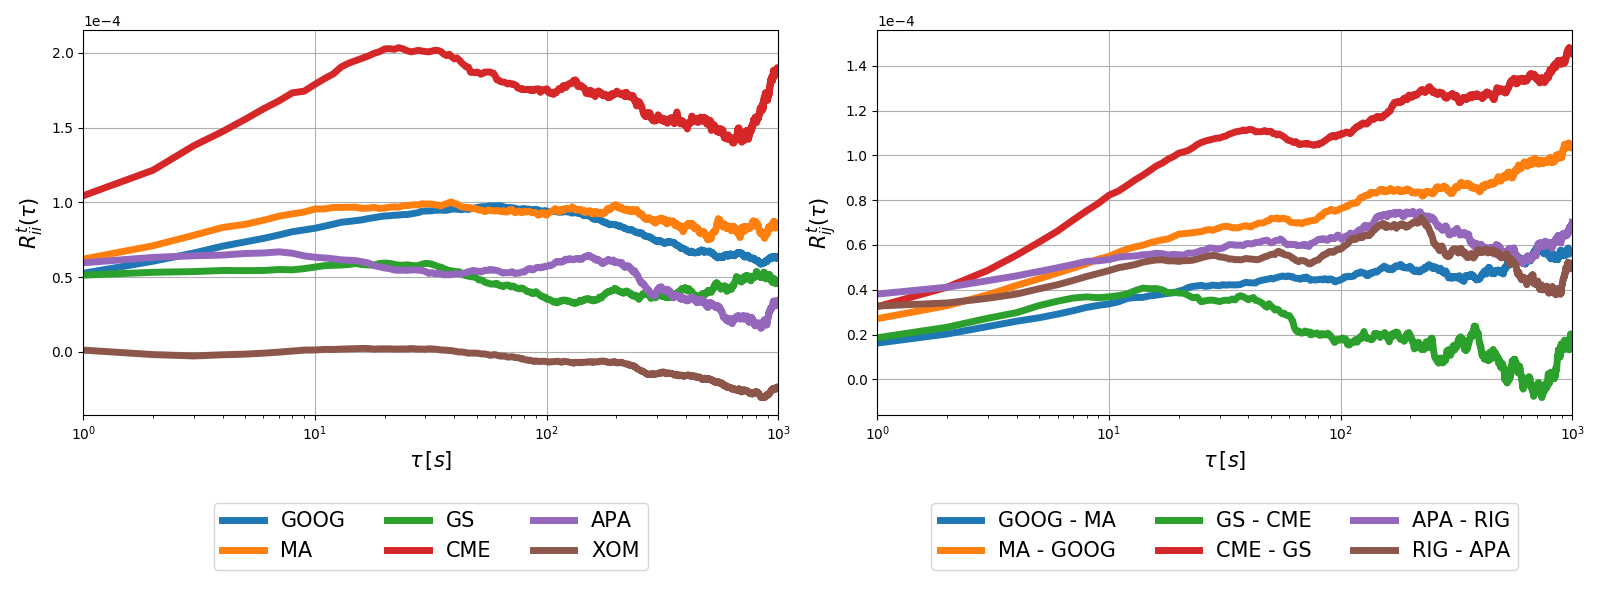
\includegraphics[width=\textwidth]
    {figures/03_responses_trade_scale_2008.png}
    \caption{Self- and cross-response functions
             $R^{t}_{ij}\left(\tau\right)$ excluding
             $\varepsilon^{t}_{j}\left(t\right) = 0$ in 2008 versus time
             lag $\tau$ on a logarithmic scale in trade time scale. Self-
             responses (left) of individual stocks and cross-response (right)
             of stock pairs from the same economic sector.}
    \label{fig:response_function_trade_scale}
\end{figure*}

The results of Fig. \ref{fig:response_function_trade_scale} show the self-
responses of the six stocks used in the analysis and the cross-responses for
pairs of stocks representing three different economic sectors. Compared with
the market response in second time scale, the market response in trade time
scale is almost one order of magnitude smaller.

%%%%%%%%%%%%%%%%%%%%%%%%%%%%%%%%%%%%%%%%%%%%%%%%%%%%%%%%%%%%%%%%%%%%%%%%%%%%%%%
\subsection{Response functions in physical time scale}
\label{subsec:response_function_physical}

One important detail to compute the market response in physical time scale is
to define how the averaging of the function will be made. This, because the
response functions highly differ when we include or exclude
$\varepsilon^{p}_j \left( t\right) = 0$ \cite{Wang_2016_cross}. The
cross-responses including $\varepsilon^{p}_j \left( t\right) = 0$ are weaker
than the excluding ones due to the omission of direct influence of the lack of
trades. However, either including or excluding
$\varepsilon^{p}_j \left( t\right) = 0$ does not change the trend of price
reversion versus the time lag, but it does affect the response function
strength \cite{Wang_2016_avg}.

Regarding the definition of the cross-response functions in- and excluding
$\varepsilon^{p}_j \left( t\right) = 0$, the general averaging is

\begin{equation}\label{eq:response_inc}
    R_{ij}^{\left(\text{inc. }0\right)}\left(\tau\right)=
    \frac{\sum_{t=1}^{T_{j}+T_{j,n}} r^{p}_{i}\left(t - 1,\tau\right)
    \cdot\varepsilon_{j}^{p}\left(t \right)}{T_{j}+T_{j,n}}
\end{equation}

\begin{equation}\label{eq:response_exc}
    R_{ij}^{\left(\text{exc. }0\right)}\left(\tau\right)=
    \frac{\sum_{t=1}^{T_{j}} r^{p}_{i}\left(t - 1,\tau\right)
    \cdot\varepsilon_{j}^{p} \left(t\right)}{T_{j}}
\end{equation}

Where the superscript inc. and exc. refers to including and excluding
$\varepsilon^{p}_j \left( t\right) = 0$. For stock $j$, $T_j$  is the total
trading time of stock $j$ and $T_{j,n}$ is the total time of lack of trading or
buy sell balance. The numerators in Eqs. \ref{eq:response_inc} and
\ref{eq:response_exc} are the same, while the denominators differ
\cite{Wang_2016_avg}.

Hence,

\begin{equation}\label{eq:relation_response_inc_exc}
    R_{ij}^{\left(\text{inc. }0\right)}\left(\tau\right)=f_{j}
    \cdot R_{ij}^{\left(\text{exc. }0\right)}\left(\tau\right)
\end{equation}

Where the relative trading frequency is defined as \cite{Wang_2016_avg}

\begin{equation}\label{eq:response_trading_frequency}
    f_{j}=\frac{T_{j}}{T_{j}+T_{j,n}}
\end{equation}

The most frequently traded stocks have $f_{i} = 1$, because the time $T_{j,n}$
is zero. According to Eq. \ref{eq:relation_response_inc_exc}, the
cross-response including $\varepsilon^{p}_j \left( t\right) = 0$ is the one
excluding $\varepsilon^{p}_j \left( t\right) = 0$ scaled by a proper
probability.

Then, we will only take in account the cross-response function excluding
$\varepsilon^{p}_j \left( t\right) = 0$.

We define the self- and cross-response functions in physical time scale, using
the trade signs and the returns in physical time scale. The response is

\begin{equation}\label{eq:response_functions_time_scale_general}
    R^{p}_{ij}\left(\tau\right)=\left\langle r^{p}_{i}\left(t-1, \tau\right)
    \cdot\varepsilon_{j}^{p} \left(t\right)
    \right\rangle _{p}
\end{equation}

And the corresponding explicit expression reads

\begin{align}\label{eq:response_seconds_explicit}
    R_{ij}^{p}\left(\tau\right)&=\frac{1}{\sum_{d=d_{0}}^{d_{f}}
    \sum_{t=t_{0}}^{t_{f}} \eta\left[ \varepsilon_{j,d}^{p}
    \left(t\right)\right]} \nonumber \\
    &\cdot\sum_{d=d_{0}}^{d_{f}} \sum_{t=t_{0}}^{t_{f}}
    r^{p}_{i,d}\left(t-1,\tau\right) \cdot\varepsilon_{j,d}^{p}\left(t\right)
    \cdot\eta\left[\varepsilon_{j}^{p} \left(t\right)\right] \\
    &=\sum_{d=d_{0}}^{d_{f}}\sum_{t=t_{0}}^{t_{f}}r^{p}_{i,d}
    \left(t-1,\tau\right) \cdot\frac{\varepsilon_{j,d}^{p}\left(t\right)
    \cdot\eta\left[\varepsilon_{j,d}^{p} \left( t\right)\right]}
    {\sum_{d=d_{0}}^{d_{f}}\sum_{t=t_{0}}^{t_{f}}\eta
    \left[\varepsilon_{j,d}^{p} \left(t\right)\right]} \nonumber \\
    &=\sum_{d=d_{0}}^{d_{f}}\sum_{t=t_{0}}^{t_{f}}r^{p}_{i,d}
    \left(t-1,\tau\right) \cdot\text{sgn}\left(E_{j,d}\left(t\right)\right)
    \cdot w_{j,d}^{p}\left(t\right)
\end{align}

Where

\begin{equation}
    \eta\left(x\right)=\left\{ \begin{array}{cc}
    1, & \text{If }x\ne0 \\
    0, & \text{otherwise}
    \end{array}\right.
\end{equation}

take only in account the seconds with trades and
\begin{equation}
    w_{j,d}^{p}\left(t\right) = \frac{\eta\left[\text{sgn}
    \left(E_{j,d}\left( t\right)\right)\right]}{\sum_{d=d_{0}}^{d_{f}}
    \sum_{t=t_{0}}^{t_{f}} \eta\left[\text{sgn}\left(E_{j,d}
    \left(t\right)\right)\right]}
\end{equation}

is a weight function that depends on the normalization of the response.

\begin{figure*}[htbp]
    \centering
    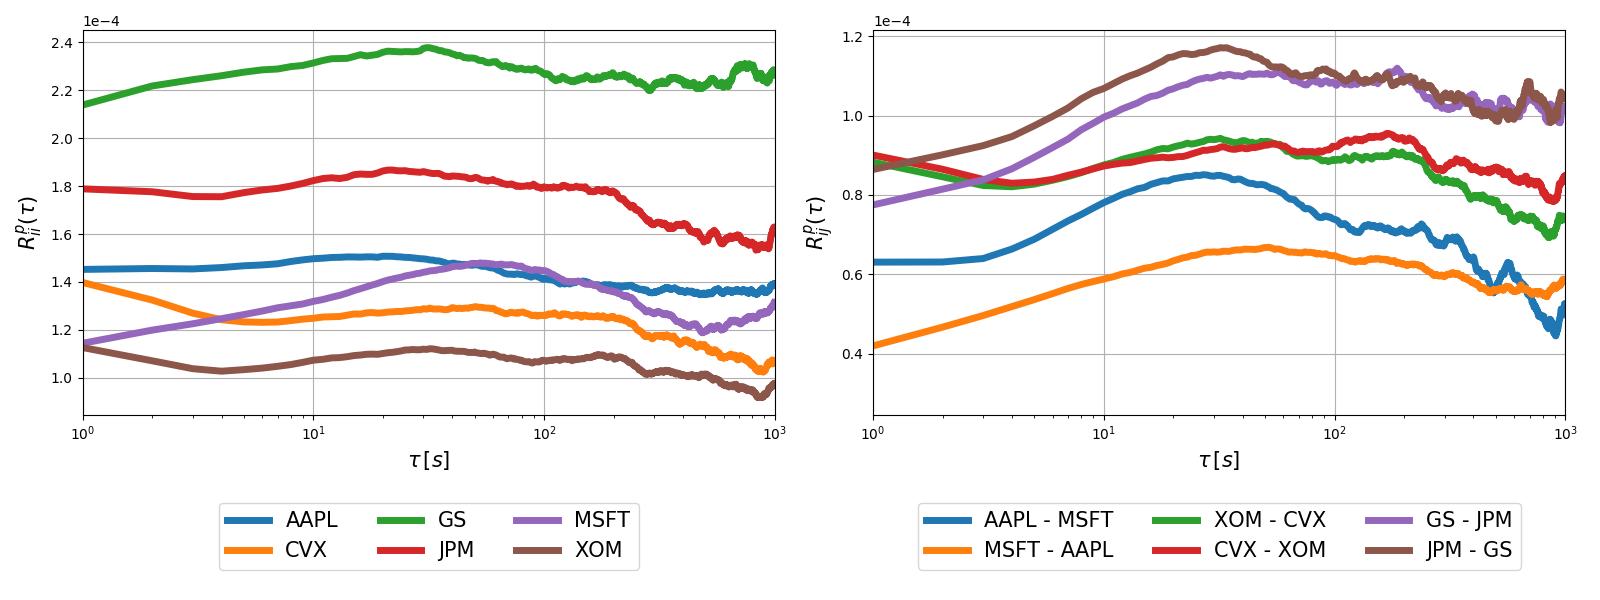
\includegraphics[width=\textwidth]
    {figures/03_responses_physical_scale_2008.png}
    \caption{Self- and cross-response functions $R^{p}_{ij}\left(\tau\right)$
             excluding $\varepsilon^{p}_{j}\left(t\right) = 0$ in 2008 versus
             time lag $\tau$ on a logarithmic scale in second time scale.
             Self-responses (left) of individual stocks and cross-response
             (right) of stock pairs from the same economic sector.}
    \label{fig:market_response_time_scale}
\end{figure*}

The results showed in Figure \ref{fig:market_response_time_scale} are identical
with the ones showed in \cite{Wang_2016_cross} for the same data. We can say
again that in all cases, an increase to a maximum is followed by a decrease,
i.e. the trend in the self- and cross-response is eventually reversed.

%%%%%%%%%%%%%%%%%%%%%%%%%%%%%%%%%%%%%%%%%%%%%%%%%%%%%%%%%%%%%%%%%%%%%%%%%%%%%%%
\subsection{Activity response functions in physical time scale}
\label{subsec:activity_response_function}

Finally, we define the activity self- and cross-response functions in physical
time scale, using the trade signs and the returns in physical time scale.
We add a factor $N_{j,d} \left(t \right)$ to check the influence of the
frequency of trades in a second in the response functions. The activity
response is

\begin{equation}\label{eq:activity_response_functions_general}
    R^{a}_{ij}\left(\tau\right)=\left\langle r^{p}_{i}\left(t-1, \tau\right)
    \cdot\varepsilon_{j}^{p} \left(t\right) \cdot N \left(t \right)
    \right\rangle _{p}
\end{equation}

And the corresponding explicit expression reads

\begin{align}
    R_{ij}^{a}\left(\tau\right)&=\frac{1}{\sum_{d=d_{0}}^{d_{f}}
    \sum_{t=t_{0}}^{t_{f}}N_{j,d} \left(t\right)} \nonumber \\
    &\cdot\sum_{d=d_{0}}^{d_{f}}\sum_{t=t_{0}}^{t_{f}}r^{p}_{i,d}
    \left(t-1,\tau\right) \cdot\varepsilon_{j,d}^{p}\left(t\right)\cdot N_{j,d}
    \left(t\right)\\
    &=\sum_{d=d_{0}}^{d_{f}} \sum_{t=t_{0}}^{t_{f}}r^{p}_{i,d}
    \left(t-1,\tau\right) \cdot\frac{\varepsilon_{j,d}^{p}\left(t \right)
    \cdot N_{j,d}\left(t\right)} {\sum_{d=d_{0}}^{d_{f}}\sum_{t=t_{0}}^{t_{f}}
    N_{j,d}\left(t \right)} \nonumber \\
    &=\sum_{d=d_{0}}^{d_{f}} \sum_{t=t_{0}}^{t_{f}}r^{p}_{i,d}
    \left(t-1,\tau\right) \cdot\text{sgn}\left(E_{j,d}\left(t\right)\right)
    \cdot w_{j,d}^{a}\left(t\right)
\end{align}

Where

\begin{equation}
    w_{j,d}^{a}\left(t\right) = \frac{N_{j,d}\left(t \right)}
    {\sum_{d=d_{0}}^{d_{f}}\sum_{t=t_{0}}^{t_{f}}N_{j,d}\left(t\right)}
\end{equation}

is a weight function that depends on the normalization of the response.

As $E_{j,d}\left(t\right)$ is the sum of $+1$ and $-1$ in one second and
$N_{j,d}\left(t\right)$ is the number of trades in a second,
$N_{j,d}\left(t\right) \ge E_{j,d}\left(t\right)$.
$N_{j,d}\left(t\right) = E_{j,d}\left(t\right)$ only when all the trades in a
second are buys $(+1)$.

The trade weight reduces noises, The physical weight gives every step the same
weight, and the activity weight emphasizes seconds with large activity.

In Figure \ref{fig:relation_responses}, we can see how the three
responses have approximately the same shape, but the strength of the signal
varies depending on the definition. The frequency of trades have a large
influence in the responses.

\begin{figure*}[htbp]
    \centering
    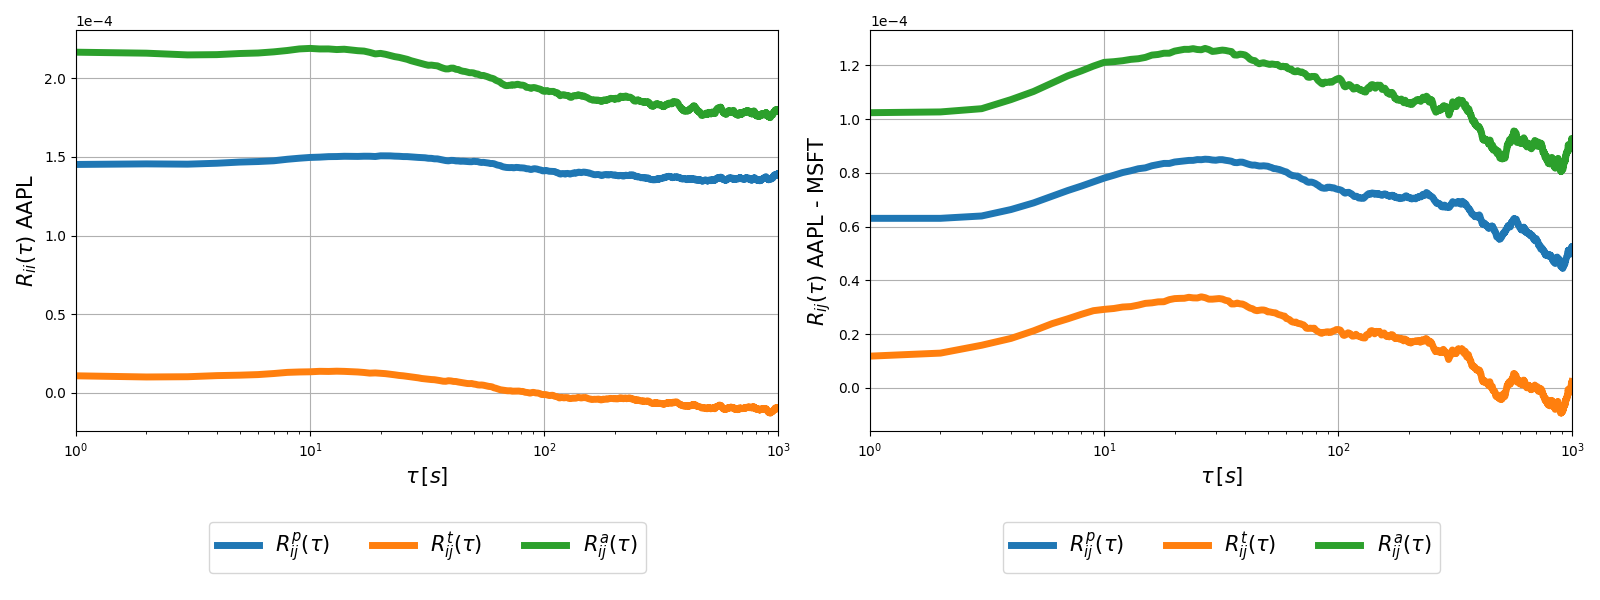
\includegraphics[width=\textwidth]
    {figures/03_response_comparison_2008_AAPLi_MSFTj.png}
    \caption{Self- and cross-response functions
             $R^{scale}_{ij}\left(\tau\right)$ excluding
             $\varepsilon^{p}_{j}\left(t\right) = 0$ in 2008 versus time lag
             $\tau$ on a logarithmic scale. a) self-response function of Apple
             Inc. stock, b) cross-response function of Apple Inc-Microsoft
             Corp. stocks.}
    \label{fig:relation_responses}
\end{figure*}

As predicted by the weights, the event response is weaker than the physical
response, and the activity response is the strongest response.
\section{Time shift}
\section{Short and long response functions}\label{sec:short_long}

Regarding Equation \ref{eq:return_general}, we use a time lag $\tau$ in the
returns to see the gains or loses in a future time. However, the strenght of the return in the time lag
should not be equal along its length. Then, we divide the full range time lag $\tau$ in an
immediate time lag and in a late time lag as show in Fig. \ref{fig:tau_short_long}, where

\begin{equation}\label{eq:tau_short_long}
    \tau = \tau' + \left( \tau - \tau' \right)
\end{equation}

for $\tau' < \tau$. This distinguish the returns depending in the time lag as
the short (immediate) return $\tau'$ with the long return $\tau - \tau'$.

\begin{figure}[htbp]
    \centering
    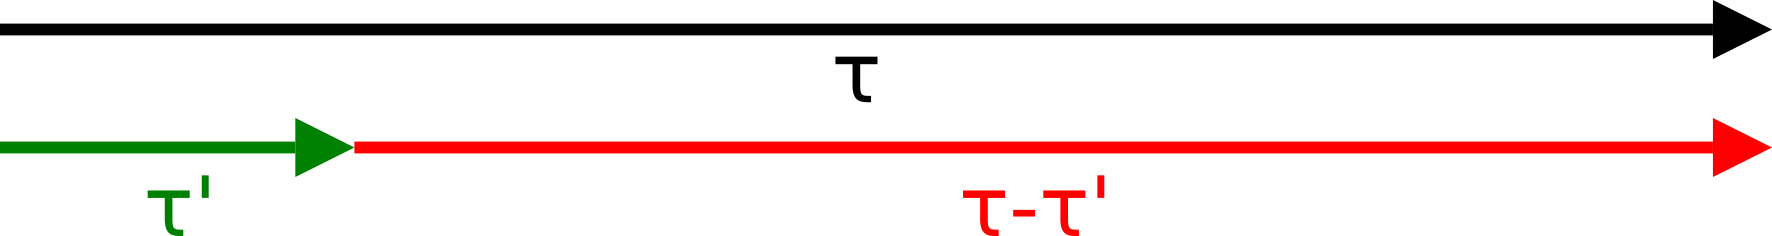
\includegraphics[width=\columnwidth]{figures/05_tau_short_long.png}
    \caption{$\tau$ value divided in short and long time lag.}
    \label{fig:tau_short_long}
\end{figure}

To use the short and long time lag, we rewrite the returns in physical
time scale as

\begin{align}\label{eq:short_long_return}
    r^{sl,p}_{i}\left(t,\tau\right)&=\ln\left(\frac{m_{i}\left(t+\tau\right)}
    {m_{i} \left(t\right)}\right) \nonumber \\
    &=\ln\left(\frac{m_{i}\left(t+\tau\right)}{m_{i}\left(t+\tau'\right)}
    \cdot\frac{m_{i} \left(t+\tau'\right)}{m_{i}\left(t\right)}\right)
    \nonumber \\
    &=\ln\left(\frac{m_{i}\left(t+\tau\right)}{m_{i}\left(t+\tau'\right)}
    \right)+ \ln\left(\frac{m_{i}\left(t+\tau'\right)}{m_{i}\left(t\right)}
    \right)\nonumber \\
    &\approx\frac{m_{i}\left(t+\tau\right)-m_{i}\left(t+\tau'\right)}
    {m_{i}\left(t+\tau'\right)} +\frac{m_{i}\left(t+\tau'\right)-m_{i}
    \left(t\right)}{m_{i}\left(t\right)}
\end{align}

where $sl$ refers to short-long and the second term of the right part is constant with respect to $\tau$.
Replacing Equation \ref{eq:short_long_return} in the response function (Eq. \ref{eq:response_functions_time_scale_general}) we have

\begin{align}\label{eq:short_long_response}
    R^{sl,p}_{ij}\left(\tau\right)&=\left\langle r^{sl,p}_{i}\left(t - 1, \tau\right)
    \cdot\varepsilon^{p}_{j}\left(t\right)\right\rangle _{p} \nonumber \\
    &\approx\left\langle \frac{m_{i}\left(t - 1 +\tau\right)-m_{i}
    \left(t - 1 +\tau'\right)} {m_{i}\left(t - 1 +\tau'\right)}\cdot\varepsilon_{j}
    \left(t\right)\right\rangle _{p} \nonumber \\
    & +\left\langle \frac{m_{i}
    \left(t - 1 +\tau'\right)-m_{i}\left(t - 1\right)}{m_{i}\left(t - 1\right)}
    \cdot\varepsilon_{j}\left(t\right)\right\rangle _{p}
\end{align}

Where the first term in the right side of Equation \ref{eq:short_long_response}
is the long response and the right term is the short response. Again, the right
term of Equation \ref{eq:short_long_response} is independent of $\tau$.

\begin{figure*}[htbp]
    \centering
    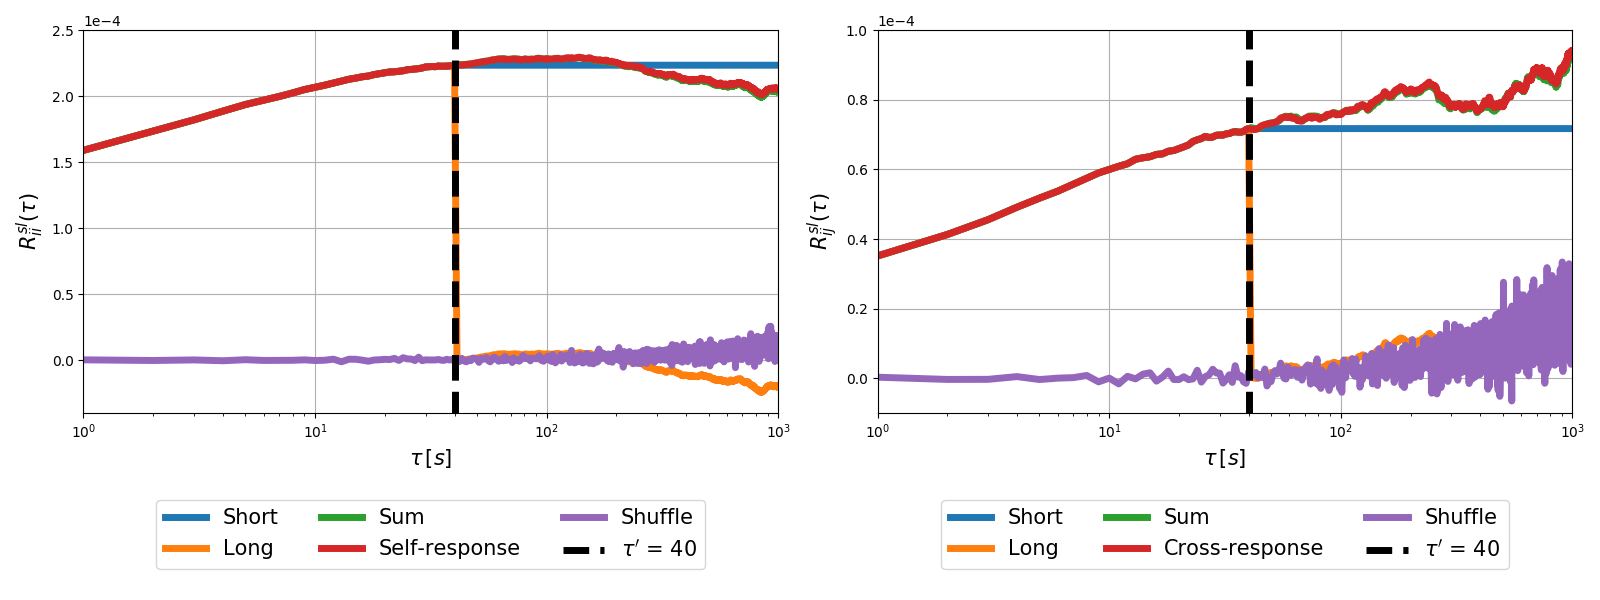
\includegraphics[width=\textwidth]
    {figures/05_short_long_GOOG_MA.png}
    \caption{Self- and cross-response functions $R^{p}_{ij}\left(\tau\right)$ excluding
            $\varepsilon^{p}_{j}\left(t\right) = 0$ in 2008 versus time lag $\tau$ on a
            logarithmic scale using a $\tau'=40$. a) self-response function of Apple Inc. stock,
            b) cross-response function of Apple Inc-Microsoft Corp. stocks.}
    \label{fig:short_long_responses}
\end{figure*}

The results in Fig. \ref{fig:short_long_responses} show the short response, the
long response, the addition of the short response and long response (Sum), the
original response, a random response and the value of $\tau'$.

The main signal of the response function come from the short response. Depending
on the stock and the value of $\tau'$ the long response can increase or decrease
the short response signal, but in general the long response does not give a
significant contribution to the complete response.

Before $\tau'$, the short response and long response are the same, as the self
and cross-response definition do not define values smaller
than $\tau '$, so it is computed as the original response. In the figure, the
curves of the short and long response are under the curve of the original response. After $\tau'$, the
short response is a strong constant signal. On the other hand, the long
response immediately fades, showing the small contribution to the final
response. To compare the significance of the long response, We added a random
response made with the trade signs used to compute the response but with a
shuffle order. The long response and the random response are comparable, and
show how the long response is not that representative in the final response.
If we add the short and long response, we obtain the original response. In Fig.
\ref{fig:short_long_responses}, the original response (red line) has the same
shape to the addition of the short and long response (green line).

For the response functions that show the increase-decrease behavior in between
the time lag $\tau = 10^{3}$, the peak is usually between $\tau = 10^{1}$ and
$\tau = 10^{2}$. In these cases the long response is always negative after the
$\tau'$ value and is comparable in magnitude with the random signal.

On the other hand, the response functions that requires a bigger time lag to
show the increase-decrease behavior, have non negative long responses, but still
they are comparable in magnitude with the random signal.

\section{Conclusion}

\section{Author contribution statement}

TG proposed the research. SMK and JCHL developed the method of analysis.
The idea to look the time shift was due to JCHL, and the idea of the time lag
analysis was due to SMK. JCHL carried out the analyisis. All the authors
contributed equally to analyze the results and write the paper.

\begin{acknowledgement}
    One of us (JCHL) acknowledges financial support from the German
    Academic Exchange Service (DAAD) with
    the program ``Research Grants - Doctoral Programmes in Germany''
    (Funding programme 57381412)
\end{acknowledgement}


\bibliographystyle{plain}
\bibliography{bib}

\end{document}
